%task analasys
\section{Task decomposition analysis}
\justify
In this section we are going to take a look into the task decomposition analysis of the nqueens algorithm.
\justify
First of all we runned a tareador instrumented version of the code. Which gave the following output.
\begin{figure}[!h]
    \centering
    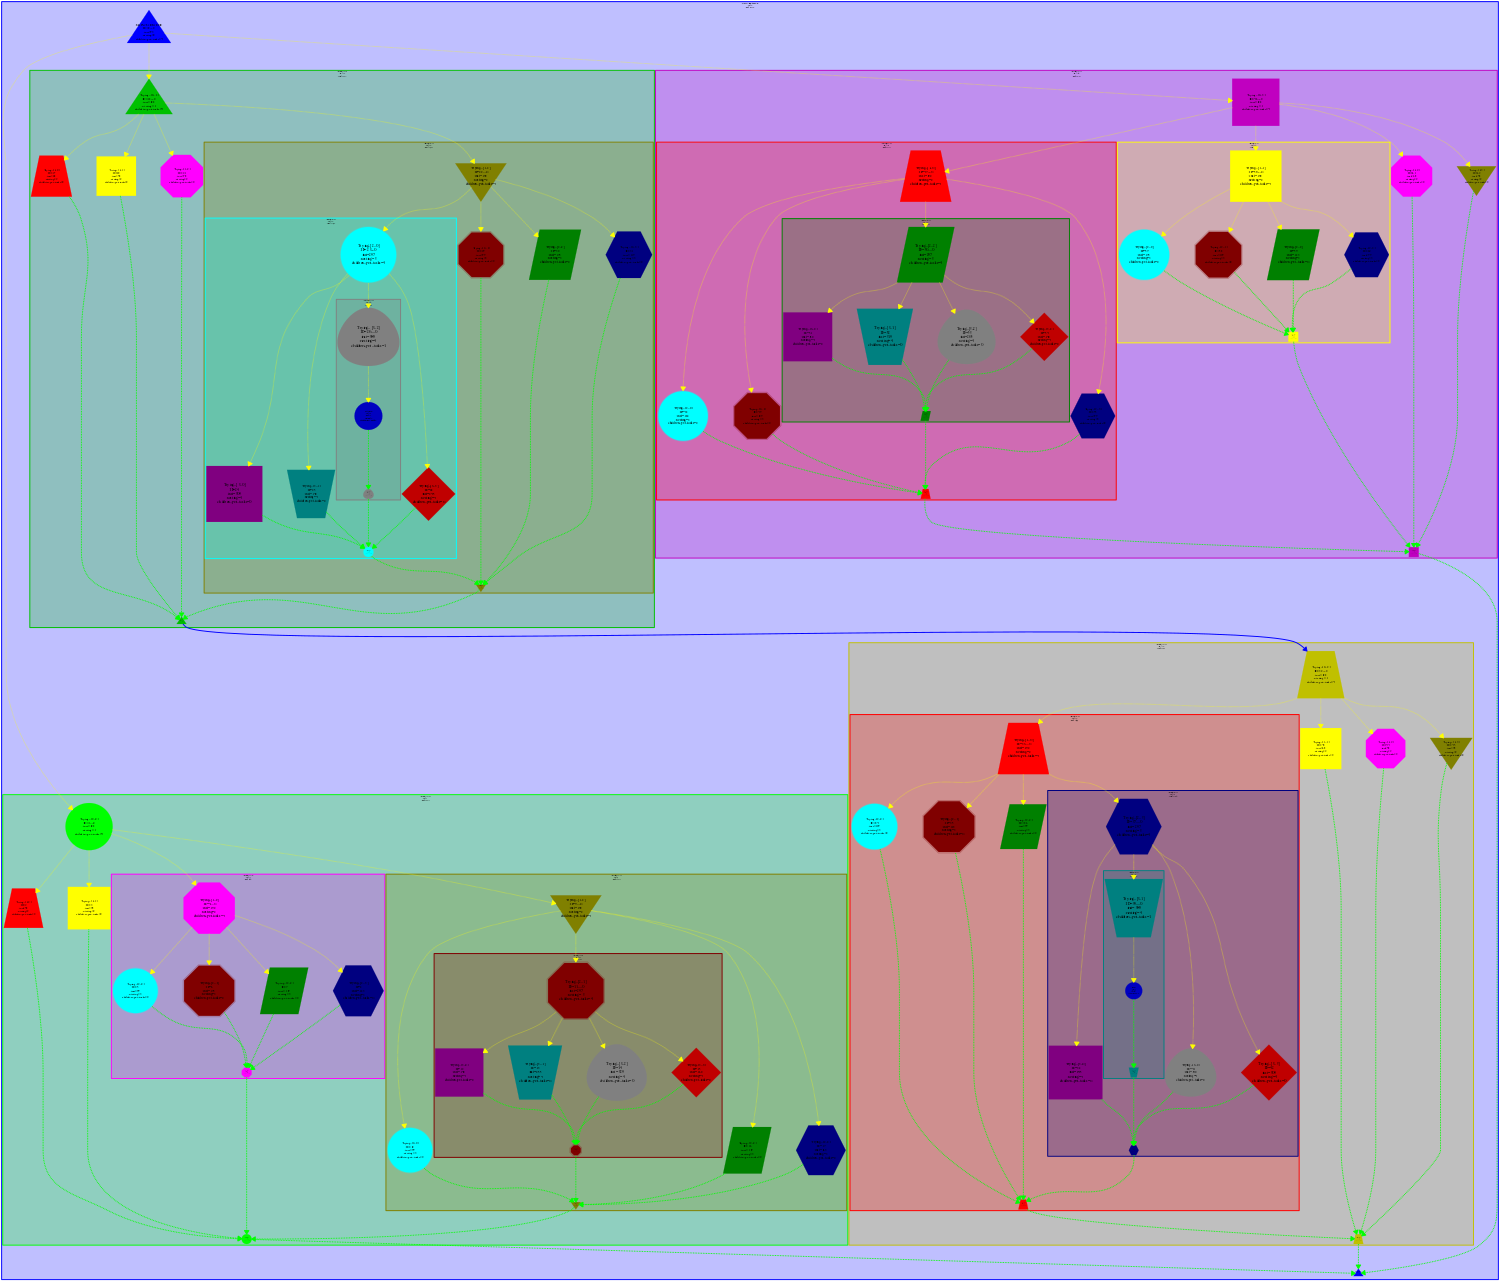
\includegraphics[width=0.78\textwidth]{dependency_graph.png}
    \caption{Strong speed-up plots}
    \label{fig:tareador}
\end{figure}
\justify
From the dependency graph we can visually observe the execution of the backtracking algorithm. Also we observe only dependencies between a call to nqueens and the function that calls it, as they share the vector \texttt{char *a}. We must take that into account for our future parallel implementations. 
\justify
Another thing that we observe from the graph is that for each recursion level we create a lot of tasks. We probably will need to implement a cutoff mechanism to reduce overheads due to task creation and work distribution.

